\documentclass[12pt]{report}

\usepackage[round]{natbib}
\usepackage[margin=1in]{geometry}
\usepackage{amsmath,amssymb,amsfonts}
\usepackage{algorithmic}
\usepackage{graphicx}
\usepackage{textcomp}
\usepackage{xcolor}
\usepackage{booktabs}
\usepackage{multirow}
\usepackage{tikz}
\usetikzlibrary{arrows.meta, positioning, shapes.geometric, fit, backgrounds}
\usepackage{url}
\usepackage{hyperref}
\hypersetup{colorlinks=false}

\def\BibTeX{{\rm B\kern-.05em{\sc i\kern-.025em b}\kern-.08em
    T\kern-.1667em\lower.7ex\hbox{E}\kern-.125emX}}

% ─────────────────────────────────────────────────────────────────────────────
% Thesis metadata (edit placeholders as needed)
% ─────────────────────────────────────────────────────────────────────────────
\newcommand{\thesistitle}{Markov-Initialized Transformers for Explainable\\Android Malware Family Classification}
\newcommand{\university}{Delhi Technological University}
\newcommand{\department}{Department of Applied Mathematics}
\newcommand{\degree}{Bachelor of Technology (B.Tech)}
\newcommand{\projecttype}{B.Tech Project Thesis}
\newcommand{\submissionmonth}{[Month]}
\newcommand{\submissionyear}{[Year]}
\newcommand{\place}{New Delhi, India}

\newcommand{\candidateone}{Arav Jain}
\newcommand{\candidatetwo}{Divyanshu Bansal}
\newcommand{\candidatethree}{Harij Sharma}
\newcommand{\candidatefour}{Anshul Arora}

\newcommand{\emailone}{aravjain\_mc22a13\_49@dtu.ac.in}
\newcommand{\emailtwo}{divyanshubansal\_mc22a14\_03@dtu.ac.in}
\newcommand{\emailthree}{harijsharma\_mc22a14\_10@dtu.ac.in}
\newcommand{\emailfour}{anshularora@dtu.ac.in}

\newcommand{\supervisor}{[Supervisor Name]}
\newcommand{\supervisordesignation}{[Designation]}
\newcommand{\hod}{[Head of Department Name]}
\newcommand{\hoddesignation}{[Designation]}

\begin{document}

% ─────────────────────────────────────────────────────────────────────────────
% Cover Page
% ─────────────────────────────────────────────────────────────────────────────
\begin{titlepage}
\thispagestyle{empty}
\begin{center}
{\Large \textbf{\university}}\\[0.2cm]
{\large \department}\\[1.5cm]

{\LARGE \textbf{\projecttype}}\\[0.75cm]
{\LARGE \textbf{\thesistitle}}\\[1.5cm]

\textbf{Submitted by}\\[0.4cm]
\begin{tabular}{ll}
\candidateone & \texttt{\emailone} \\
\candidatetwo & \texttt{\emailtwo} \\
\candidatethree & \texttt{\emailthree} \\
\candidatefour & \texttt{\emailfour} \\
\end{tabular}

\vfill
{\large \submissionmonth\ \submissionyear}\\
{\large \place}
\end{center}
\end{titlepage}

% ─────────────────────────────────────────────────────────────────────────────
% Title Page
% ─────────────────────────────────────────────────────────────────────────────
\begin{titlepage}
\thispagestyle{empty}
\begin{center}
{\LARGE \textbf{\thesistitle}}\\[1cm]

A project thesis submitted in partial fulfillment of the requirements\\
for the award of the degree of\\[0.3cm]
\textbf{\degree}\\[0.6cm]
by\\[0.4cm]

\begin{tabular}{ll}
\candidateone & [Roll No.] \\
\candidatetwo & [Roll No.] \\
\candidatethree & [Roll No.] \\
\candidatefour & [Roll No.] \\
\end{tabular}

\vfill
\textbf{Under the supervision of}\\[0.2cm]
\supervisor\\
\supervisordesignation\\
\department, \university

\vfill
{\large \submissionmonth\ \submissionyear}
\end{center}
\end{titlepage}

\pagenumbering{roman}
\setcounter{page}{1}

% ─────────────────────────────────────────────────────────────────────────────
% Candidate's Declaration
% ─────────────────────────────────────────────────────────────────────────────
\chapter*{Candidate's Declaration}
\addcontentsline{toc}{chapter}{Candidate's Declaration}

We hereby declare that the work presented in this thesis titled
\textit{\thesistitle} is an original record of our work carried out under the
supervision of \supervisor, \supervisordesignation, \department,
\university. This thesis has not been submitted, in whole or in part, for the
award of any other degree or diploma.

\vspace{1cm}
\noindent Place: \place \\
Date: [Date]

\vspace{1cm}
\begin{flushright}
\begin{tabular}{l}
\candidateone \\
\candidatetwo \\
\candidatethree \\
\candidatefour \\
\end{tabular}
\end{flushright}

% ─────────────────────────────────────────────────────────────────────────────
% Certificate
% ─────────────────────────────────────────────────────────────────────────────
\chapter*{Certificate}
\addcontentsline{toc}{chapter}{Certificate}

This is to certify that the thesis titled \textit{\thesistitle} has been
carried out by \candidateone, \candidatetwo, \candidatethree, and
\candidatefour under my supervision in partial fulfillment of the
requirements for the award of the degree of \degree from \university.
The work reported herein is genuine and has not been submitted for any
other degree or diploma.

\vspace{1cm}
\noindent Place: \place \\
Date: [Date]

\vspace{1cm}
\noindent
\begin{tabular}{p{0.45\textwidth}p{0.45\textwidth}}
\textbf{Supervisor} & \textbf{Head of Department} \\
\supervisor & \hod \\
\supervisordesignation & \hoddesignation \\
\end{tabular}

% ─────────────────────────────────────────────────────────────────────────────
% Abstract
% ─────────────────────────────────────────────────────────────────────────────
\chapter*{Abstract}
\addcontentsline{toc}{chapter}{Abstract}

Mobile malware sandboxes generate rich API call traces that capture true
runtime behavior, but the deep learning models that classify these traces
offer little insight into their decisions.
This study explores whether embedding initialization can make a Transformer's own
attention mechanism more interpretable.
The proposed approach builds a global multi-step API transition matrix,
factorizes it via Truncated SVD, and uses the resulting vectors to
initialize the model's token embeddings prior to supervised training,
encoding global behavioral structure into the embedding space from the
outset.
To measure the effect on transparency, a deletion test is utilized: if masking
the tokens that the \textit{[CLS]} attention map ranks highest causes a
larger confidence drop than masking random tokens, the attention is
meaningfully aligned with the model's actual decision.
Against a plain randomly-initialized Transformer on 9,337 Droidmon
execution traces across 8 Android malware families, the Markov-initialized
variant shows a substantially larger faithfulness gap (27.1\% vs.\ 17.0\%),
with a modest 2.6\,pp Macro-F1 cost.
A per-family breakdown reveals that the gain is concentrated in families
with stereotyped API chains and absent for parasitic malware that blends
into host-app traffic, offering a principled account of where structural
initialization helps.

\textbf{Keywords:} Android malware classification, Transformer, explainability,
Markov chain, API call sequences, attention faithfulness

% ─────────────────────────────────────────────────────────────────────────────
% Acknowledgement
% ─────────────────────────────────────────────────────────────────────────────
\chapter*{Acknowledgement}
\addcontentsline{toc}{chapter}{Acknowledgement}

This work was supported by the Department of Applied Mathematics at Delhi Technological University.

% ─────────────────────────────────────────────────────────────────────────────
% Contents and Lists
% ─────────────────────────────────────────────────────────────────────────────
\tableofcontents
\clearpage

\listoftables
\addcontentsline{toc}{chapter}{List of Tables}
\clearpage

\listoffigures
\addcontentsline{toc}{chapter}{List of Figures}
\clearpage

\chapter*{List of Symbols, Abbreviations and Nomenclature}
\addcontentsline{toc}{chapter}{List of Symbols, Abbreviations and Nomenclature}
\begin{tabular}{ll}
\toprule
\textbf{Symbol} & \textbf{Meaning} \\
\midrule
API & Application Programming Interface \\
CLS & Classification token prepended to the sequence \\
SVD & Singular Value Decomposition \\
Macro-F1 & Macro-averaged F1-score \\
AUROC & Area Under the Receiver Operating Characteristic curve \\
PAD, UNK & Padding and unknown tokens \\
$d_{\text{model}}$ & Transformer embedding dimension \\
$k$ & Markov spacing between API calls \\
$G$ & Faithfulness gap in deletion test \\
\bottomrule
\end{tabular}

\clearpage
\pagenumbering{arabic}

% ─────────────────────────────────────────────────────────────────────────────
% Chapters
% ─────────────────────────────────────────────────────────────────────────────
\chapter{Introduction}

Android malware continues to pose a significant threat to mobile security,
with millions of new malicious samples detected annually~\citep{av_test_2023}.
Family-level classification, attributing a sample to a specific malware
family such as Airpush, DroidKungFu, or Fusob, is essential for incident
response, threat intelligence, and understanding the behavioral evolution
of malware campaigns. Family-level classification is clinically meaningful:
identifying specific families (e.g., adware vs.\ root exploits) provides
actionable remediation context that binary detection alone cannot.

Dynamic analysis via sandboxing captures actual runtime API calls rather
than static bytecode, providing traces that are robust to code obfuscation.
Deep learning models, such as CNNs and LSTMs, achieve
high accuracy on such traces but operate as black boxes. Post-hoc
explanation methods such as SHAP~\citep{lundberg2017shap} and LIME
explain a surrogate model, not the model itself. Intrinsic
explainability, where the model's own internal representations serve
as explanations, remains underexplored in the malware domain.

The \textit{[CLS]} token's attention distribution over input tokens
is a natural candidate for intrinsic explanation: it produces a
per-sample importance ranking without any external computation.
However, whether attention constitutes a \textit{faithful}
explanation, one that identifies the tokens the model genuinely
relies on, is empirically contested~\citep{jain2019attention,
wiegreffe2019attention}. Deletion tests~\citep{samek2017evaluating}
provide a concrete criterion that sidesteps the theoretical debate:
if masking the highest-attention tokens reduces model confidence
more than masking random tokens, the attention map has predictive
alignment with model behavior.

We propose to improve attention faithfulness by initializing the
Transformer's token embeddings from SVD-factorized Markov transition
matrices built from k-spaced API co-occurrences in the training set.
This injects global behavioral structure into the embedding space
before any labeled training begins. Our hypothesis is that embeddings
pre-encoded with transition dynamics will guide attention heads toward
behaviorally relevant tokens, producing more faithful explanations.

Our contributions are:
\begin{enumerate}
  \item A method for constructing Markov-initialized embeddings via SVD
    factorization of k-spaced API transition matrices, directly compatible
    with standard Transformer architectures.
  \item A controlled ablation on 9,337 samples demonstrating that this
    initialization produces measurably more faithful \textit{[CLS]}
    attention maps.
  \item A per-family faithfulness analysis revealing family-specific
    patterns and a principled discussion of the accuracy--explainability
    tradeoff.
\end{enumerate}

% ─────────────────────────────────────────────────────────────────────────────
\chapter{Literature Review, Methodology, and Results}

\section{Related Work}

\subsection{Deep Learning for Malware Classification}
Early static-analysis work represented malware as grayscale bytecode
images and applied CNNs~\citep{nataraj2011malware}. Sequence-based models
using LSTMs and GRUs on API call traces showed strong generalization to
unseen variants~\citep{ye2019deep}. More recently, Transformer
architectures have been applied to API sequence classification, exploiting
self-attention to model long-range behavioral dependencies between API
calls. None of these works directly assess the faithfulness of the
resulting attention-based explanations.

Traditional ML remains competitive in malware classification. Random
Forests~\citep{breiman2001rf}, linear SVMs, decision trees, and Gaussian
Na\"{i}ve Bayes are widely used with engineered features or rule-based
representations; BiLSTMs~\citep{hochreiter1997lstm} remain a strong
sequence baseline for ordered API traces. We therefore include both
classical and recurrent baselines to contextualize performance.

\subsection{Explainability in Security ML}
Post-hoc methods such as SHAP and LIME have been applied to malware
classifiers~\citep{lundberg2017shap}, but they explain a surrogate model
rather than the trained model itself. Recent work in explainable Android malware detection has utilized post-hoc techniques; for example, \citet{soi2024enhancing} apply SHAP to 1D-CNNs over API sequences, while \citet{wu2021why} use input gradients for LSTMs. However, these methods typically focus on single-API attributions post-training. In contrast, our approach intrinsically encodes transition patterns directly into the embedding space.

The use of attention weights as
intrinsic explanations is theoretically contested: \citet{jain2019attention} show that alternative attention
distributions can yield identical predictions, undermining the claim
that attention reveals what the model relies on; \citet{wiegreffe2019attention} argue attention can still serve
as a partial explanation under different faithfulness definitions.
Deletion tests~\citep{samek2017evaluating} provide an empirical criterion that sidesteps this debate: they measure directly
whether the tokens a model attends to are the tokens it relies on.
While gradient-based approaches~\citep{sundararajan2017integrated} or
attention rollout~\citep{abnar2020rollout} can yield more accurate saliency maps,
they require computationally expensive backward passes or multi-layer
composition at inference time. We use raw averaged CLS attention as our explanation
because it requires no additional computation and is directly
interpretable to practitioners; the deletion test then provides
empirical evidence of whether this simple explanation is meaningful.

From a systems perspective, explanation methods differ in computational
cost: gradient-based methods such as integrated
gradients~\citep{sundararajan2017integrated} and attention
rollout~\citep{abnar2020rollout} require extra backward passes or layer
composition, whereas CLS attention can be extracted during the forward
pass. In deployment scenarios like sandbox triage, this low-overhead
property motivates intrinsic attention explanations paired with
empirical validation.

\subsection{Graph-Based and Markov Approaches}
\citet{dangelo2023kspaced} model malware behavior as
k-spaced associative rules extracted from Droidmon API traces, achieving
strong classification on the same dataset we use.
GloVe~\citep{pennington2014glove} and Word2Vec~\citep{mikolov2013word2vec}
establish the broader precedent for deriving dense token embeddings from
co-occurrence matrix factorization. We are the first to bridge Markov
transition modeling with Transformer embedding initialization for malware
classification, and to measure the effect on attention faithfulness
directly via a deletion test.

Rule-graph approaches typically apply support/confidence thresholds to
prune noisy co-occurrences and then score samples using the retained
rules. This makes them interpretable but can limit expressiveness
compared to sequence models. We therefore treat MarkovPruning as a
baseline and use Markov statistics primarily as a structural prior for
embedding initialization rather than as the classifier itself.

% ─────────────────────────────────────────────────────────────────────────────
\section{Methodology}

\subsection{Data Extraction and Sanitization}
Raw Droidmon logs are stored as JSONL files (\texttt{droidmon.log}) under
\texttt{raw\_data/}. We extract a compact, ordered event stream using
\texttt{scripts/data\_extractor.py}: each line is parsed robustly (with recovery
from trailing commas), core fields are normalized (\texttt{class},
\texttt{method}, \texttt{hooked\_class}, \texttt{hooked\_method}), and
reflection is detected either via \texttt{type == reflection} or reflective
class names (e.g., \texttt{java.lang.reflect.Method}). Events are sorted by
timestamp and written to per-family directories under \texttt{extracted\_data/}
with JSONL records containing \texttt{timestamp}, \texttt{class},
\texttt{method}, \texttt{hooked\_class}, \texttt{hooked\_method}, and
\texttt{is\_reflection}. Invalid lines are skipped to keep the pipeline robust
on noisy logs.

\subsection{Preprocessing and Tokenization}
We use API call traces from the Droidmon dynamic analysis
sandbox~\citep{droidmon}. Each trace is an ordered sequence of Android API
events. Samples with fewer than 5 API calls are excluded; for the
sequence-length sweep and deletion-test analysis we further restrict to
traces with length $\geq 30$ to stabilize statistics.

We apply reflection-aware tokenization: calls resolved via Java reflection
are tagged \texttt{REFL:class.method} using \texttt{hooked\_class} and
\texttt{hooked\_method} so that reflective targets are preserved rather than
collapsed to a generic reflection token.

A vocabulary is constructed over the training set with a minimum
frequency threshold of $f_{\min}=2$, yielding $|V|=1{,}118$ unique
API tokens plus special tokens PAD and UNK (indices 0 and 1). Sequences
are padded/truncated to a fixed length $L_{\max}$ with either head or tail
truncation. A sweep over $L_{\max}\in\{256, 512, 768\}$ and truncation
$\in\{\text{head},\text{tail}\}$ shows head truncation with $L_{\max}=512$
achieves the best Macro-F1 (0.8875 $\pm$ 0.0123;
Table~\ref{tab:seq_len_sweep}), indicating that early API calls (SDK
initialization, reflection setup, permission requests) carry more
family-discriminating signal.

\subsection{Transformer Architecture}
\label{sec:arch}

Our Transformer~\citep{vaswani2017attention} (Fig.~\ref{fig:arch})
prepends a learnable \textit{[CLS]} token to every input sequence and
classifies from the CLS final hidden state.

\textbf{Architecture.}
$d_{\text{model}}=128$, $H=4$ attention heads, $N_{\text{layers}}=2$
Transformer encoder layers, feed-forward dimension $d_{\text{ff}}=256$,
dropout $p=0.15$. Classification uses a two-layer MLP over the
$d_{\text{model}}$-dimensional CLS representation. Total parameters:
$\approx$515K.

\textbf{Implementation details.}
The encoder uses pre-norm Transformer blocks (LayerNorm before attention
and feed-forward layers), learnable positional embeddings of length
$L_{\max}+1$ (to account for CLS), and attention masks that prevent
attending to PAD tokens while leaving CLS unmasked.

\textbf{Loss.}
Class-weighted cross-entropy with inverse-frequency weights addresses
the 35$\times$ imbalance between Airpush (63\% of samples) and the
two smallest families.

\textbf{Explainability.}
For each sample, we collect the per-layer, per-head CLS attention row
$\mathbf{a}^{(\ell,h)}_{\text{CLS}} \in \mathbb{R}^{L+1}$
(the row of the softmax attention matrix corresponding to the CLS
position) and average across all heads and layers to obtain a single
importance vector $\hat{\mathbf{a}} \in \mathbb{R}^{L}$ over input
tokens. This serves as the intrinsic explanation without any
post-hoc computation.

\begin{figure}[t]
\centering
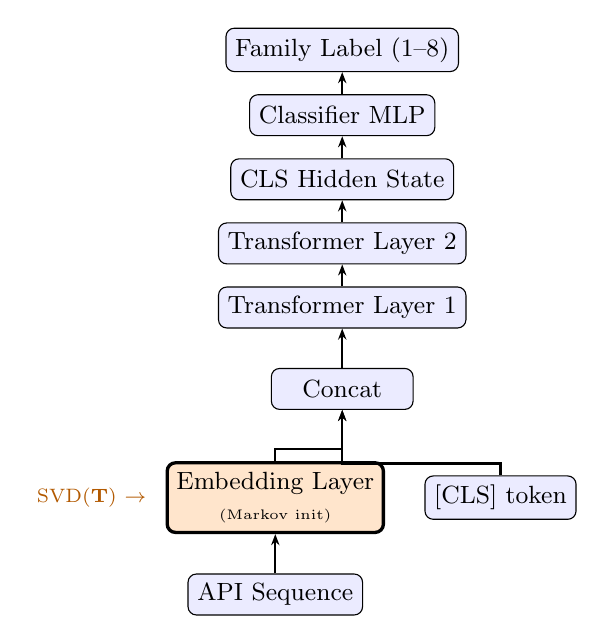
\begin{tikzpicture}[
  font=\small,
  box/.style={draw, rounded corners=3pt, minimum width=1.8cm,
              minimum height=0.52cm, align=center, fill=blue!8},
  boldbox/.style={draw, rounded corners=3pt, minimum width=1.8cm,
                  minimum height=0.52cm, align=center, fill=orange!20,
                  very thick},
  arr/.style={-{Stealth[length=4pt]}, thick},
  node distance=0.50cm and 0.0cm
]
  \node[box] (inp) {API Sequence};
  \node[boldbox, above=of inp] (emb) {Embedding Layer\\{\tiny (Markov init)}};
  \node[box, right=0.5cm of emb] (cls) {[CLS] token};
  \node[box, above=0.65cm of emb, xshift=0.85cm] (cat) {Concat};
  \node[box, above=of cat] (t1) {Transformer Layer 1};
  \node[box, above=0.28cm of t1] (t2) {Transformer Layer 2};
  \node[box, above=0.28cm of t2] (clsout) {CLS Hidden State};
  \node[box, above=0.28cm of clsout] (clf) {Classifier MLP};
  \node[box, above=0.28cm of clf] (out) {Family Label (1--8)};

  \draw[arr] (inp) -- (emb);
  \draw[arr] (cls.north) -- ++(0,0.15) -| (cat);
  \draw[arr] (emb.north) -- ++(0,0.15) -| (cat);
  \draw[arr] (cat) -- (t1);
  \draw[arr] (t1) -- (t2);
  \draw[arr] (t2) -- (clsout);
  \draw[arr] (clsout) -- (clf);
  \draw[arr] (clf) -- (out);

  \node[left=0.12cm of emb, font=\scriptsize, text=orange!70!black]
    {SVD($\mathbf{T}$) $\rightarrow$};
\end{tikzpicture}
\caption{Architecture. The embedding layer (orange) is initialized from
SVD-factorized Markov transition matrices in the proposed model.
Classification uses the CLS hidden state; CLS attention weights averaged
across all heads and layers form the intrinsic per-sample explanation.}
\label{fig:arch}
\end{figure}

\subsection{Markov Embedding Initialization}
\label{sec:markov}

\textbf{Transition matrix construction.}
For each API execution trace $\mathbf{s} = (s_1, s_2, \ldots, s_n)$ of length $n$, where each $s_i$ is an API call from vocabulary $V$, we
extract all k-spaced pairs $(s_i, s_{i+k})$ for $k \in \{1,\ldots,10\}$.
We accumulate these into a global count matrix $\mathbf{C} \in \mathbb{R}^{|V| \times |V|}$, and row-normalize to obtain the transition matrix $\mathbf{T}$:
\begin{equation}
  T_{ij} = \frac{C_{ij}}{\sum_j C_{ij}}.
\end{equation}
Using a k-spacing of $[1,10]$ captures both local and medium-range API co-occurrences, which is crucial for modeling multi-step malware behavior. A global matrix (rather than per-class matrices) is used because class labels are unavailable at inference time.

\textbf{SVD factorization.}
We apply Truncated SVD to factorize $\mathbf{T} \approx \mathbf{U}_d \boldsymbol{\Sigma}_d \mathbf{V}_d^\top$, retaining $d_{\text{model}}=128$ components. Each row of the left singular matrix $\mathbf{U}_d \in \mathbb{R}^{|V| \times d_{\text{model}}}$ encodes an API's behavioral context as a dense vector. Thus, APIs that share similar outgoing transition profiles (like the constituent calls of an SMS-fraud sequence) receive geometrically proximate embedding vectors. This provides a structural inductive bias toward attending to semantically coherent API groups before training begins, analogous to GloVe~\citep{pennington2014glove}.

\textbf{Initialization.}
The rows of $\mathbf{U}_d$ are copied into the Transformer's
\texttt{nn.Embedding} layer as initial weights; the PAD embedding is
zeroed. The embedding layer is then frozen for 5 epochs; forcing
attention heads to learn to read the pre-encoded structure; before
unfreezing for end-to-end fine-tuning.

\subsection{Faithfulness Deletion Test}
\label{sec:deletion}

We evaluate whether the averaged CLS attention map $\hat{\mathbf{a}}$
faithfully identifies the tokens the model relies on for its prediction.
For each test sample $(\mathbf{x}, y)$:
\begin{enumerate}
  \item Compute baseline probability $P_0 = P(y \mid \mathbf{x})$.
  \item Rank tokens by descending $\hat{\mathbf{a}}$; select top-$m$
    indices $\mathcal{I}_{\text{attn}}$.
  \item Mask $\mathcal{I}_{\text{attn}}$ by replacing with PAD;
    re-run inference to obtain $P_{\text{attn}}$.
  \item Repeat with $m$ uniformly random indices to obtain $P_{\text{rand}}$.
\end{enumerate}
The \textit{faithfulness gap}
$G = (P_0 - P_{\text{attn}}) - (P_0 - P_{\text{rand}})$
measures how much more the model relies on its high-attention tokens
than on random ones. We evaluate at $m \in \{5, 10, 20\}$ and report
means over 30 samples per family (240 total). $G > 0$ is a necessary,
but not sufficient, condition for faithful explanation.

\subsection{Training Protocol}
Both the plain and Markov-initialized Transformers use identical
configurations: AdamW optimizer (learning rate $5 \times 10^{-4}$,
weight decay $10^{-4}$), batch size 32, cosine annealing with
$T_{\max}=100$ epochs, gradient clipping at 1.0, and early stopping with
patience 20 on validation Macro-F1. Class imbalance is handled with
class-weighted cross-entropy using $w_c = N / (C \cdot N_c)$. For the
Markov model, the embedding layer is frozen for the first 5 epochs and
then unfrozen for end-to-end fine-tuning.
We use 3-fold stratified cross-validation with a fixed random seed (42)
and run on the best available device (MPS, CUDA, or CPU). The SVD
embedding dimension used is $d_{\text{model}}=128$.

% ─────────────────────────────────────────────────────────────────────────────
\section{Experimental Setup}
\label{sec:setup}

\subsection{Dataset}
We use the Droidmon execution traces from \citet{dangelo2023kspaced}, obtained directly from the authors.
Samples with trace length $< 5$ API calls are excluded, yielding 9,337
traces across 8 malware families (Table~\ref{tab:dataset}). The corpus
exhibits a 35$\times$ class imbalance between the dominant family
(Airpush, 63\%) and the two smallest (Fusob and SmsPay, $<2\%$ each).
Class-weighted loss and stratified fold assignment mitigate this imbalance.

Our methodology relies on dynamic API traces, which capture runtime behavior and obfuscation resistance, differentiating it from static-feature datasets like Drebin~\citep{drebin2014} or CICAndMal2017~\citep{lashkari2018cicandmal2017}. However, evaluating on a single dataset remains a limitation; future work must verify generalization to other benchmarks.

\begin{table}[t]
\centering
\caption{Dataset: Droidmon traces from \citet{dangelo2023kspaced}.}
\label{tab:dataset}
\begin{tabular}{lrl}
\toprule
\textbf{Family} & \textbf{Samples} & \textbf{Primary Behavior} \\
\midrule
Airpush      & 5,880 & Aggressive adware, user tracking \\
DroidKungFu  & 1,257 & Root exploit, data exfiltration \\
Opfake       &   596 & SMS fraud, code packing \\
GinMaster    &   523 & Backdoor, privilege escalation \\
Jisut        &   430 & Ransomware + SMS fraud \\
Genpua       &   312 & Premium SMS fraud \\
SmsPay       &   173 & Premium SMS fraud \\
Fusob        &   166 & Ransomware \\
\midrule
\textbf{Total} & \textbf{9,337} & \\
\bottomrule
\end{tabular}
\end{table}

\subsection{Baselines}
We compare against Random Forest~\citep{breiman2001rf} (200 trees),
LinearSVM (max\_iter=5000, dual=False), Decision Tree, Gaussian
Na\"{i}ve Bayes (GNB), and a 2-layer BiLSTM~\citep{hochreiter1997lstm}
($d=128$, mean-pooled). We also include the MarkovPruning rule-based
classifier from \citet{dangelo2023kspaced}, which scores k-spaced
associative rules with support/confidence pruning and softmax ranking.
Classical baselines use fixed-length API-gram features (TF-IDF in our
pipeline), while neural models operate directly on the padded sequences;
all models use the same 3-fold splits for fairness. A sweep over
MarkovPruning thresholds identifies the best operating point at
\texttt{min\_support}=$10^{-4}$, \texttt{min\_confidence}=0.8, and uniform
class weights, retaining about 3,191 rules (Table~\ref{tab:markov_sweep}).

\subsection{MarkovPruning Sweep}
We sweep the MarkovPruning baseline over support, confidence, and
class-weighting settings using the same 3-fold splits. The best operating
point is shown in Table~\ref{tab:markov_sweep}; it is reported alongside
other baselines in the main results table.

\begin{table}[t]
\centering
\caption{Best operating point for MarkovPruning (3-fold CV sweep).}
\label{tab:markov_sweep}
\begin{tabular}{lc}
\toprule
\textbf{Setting / Metric} & \textbf{Value} \\
\midrule
\texttt{min\_support} & $1\times 10^{-4}$ \\
\texttt{min\_confidence} & 0.8 \\
\texttt{class\_weights} & uniform \\
Rules kept (mean) & 3{,}191 \\
Accuracy & 0.8290 $\pm$ 0.0257 \\
Macro-F1 & 0.7250 $\pm$ 0.0272 \\
Macro-AUROC & 0.9477 $\pm$ 0.0080 \\
\bottomrule
\end{tabular}
\end{table}

\subsection{Metrics}
We report Macro-F1 (primary), Accuracy, and Macro-AUROC as
mean\,$\pm$\,std over 3 folds. Macro-F1 averages per-class F1 scores
without weighting by support, preventing the dominant Airpush class
from masking minority-family performance.

\subsection{Sequence Length and Truncation Sweep}
We evaluate $L_{\max}\in\{256, 512, 768\}$ and truncation
$\in\{\text{head},\text{tail}\}$ on the len$\geq$30 subset
(8{,}085 samples) with the same architecture and 3-fold CV. The best
configuration is $L_{\max}=512$ with head truncation, which we use for
the final training runs (Table~\ref{tab:seq_len_sweep}).

\begin{table}[t]
\centering
\caption{Sequence length and truncation sweep (len$\geq$30 subset, 3-fold CV).}
\label{tab:seq_len_sweep}
\begin{tabular}{l l c c c}
\toprule
\textbf{$L_{\max}$} & \textbf{Trunc.} & \textbf{Macro-F1} & \textbf{Accuracy} & \textbf{AUROC} \\
\midrule
512 & head & 0.8875 $\pm$ 0.0123 & 0.9445 $\pm$ 0.0053 & 0.9834 $\pm$ 0.0016 \\
768 & head & 0.8867 $\pm$ 0.0033 & 0.9459 $\pm$ 0.0059 & 0.9843 $\pm$ 0.0016 \\
256 & head & 0.8811 $\pm$ 0.0066 & 0.9410 $\pm$ 0.0031 & 0.9865 $\pm$ 0.0012 \\
512 & tail & 0.8697 $\pm$ 0.0126 & 0.9352 $\pm$ 0.0031 & 0.9805 $\pm$ 0.0034 \\
256 & tail & 0.8587 $\pm$ 0.0026 & 0.9307 $\pm$ 0.0065 & 0.9810 $\pm$ 0.0024 \\
\bottomrule
\end{tabular}
\end{table}

% ─────────────────────────────────────────────────────────────────────────────
\section{Results and Discussion}

\begin{figure*}[tp]
\centering

\includegraphics[width=0.48\textwidth]{results/figures/cls_attn_heatmap_per_family.png}
\hfill

\includegraphics[width=0.48\textwidth]{results/figures/markov_transformer_cls_attn_heatmap_per_family.png}
\caption{Average \textit{[CLS]} attention heatmaps across families for the Plain Transformer (left) and Markov-initialized Transformer (right). The Markov model strongly focuses on specific API chains for families like SmsPay and DroidKungFu, while struggling with parasitic malware like GinMaster where host-app noise dominates the transition matrix.}
\label{fig:attention_heatmaps}
\end{figure*}

\subsection{Classification Performance}

Table~\ref{tab:classification} reports 3-fold stratified CV results for
all models, including the MarkovPruning rule-based baseline. The Plain
Transformer achieves Macro-F1\,=\,0.884, within 1\,pp of the top performer
(BiLSTM, 0.894) and comparable to Random Forest (0.893). It outperforms
MarkovPruning by roughly 17.5\,pp in Macro-F1, indicating that sequence
models capture richer behavior than pruned rule graphs on this corpus.

The Markov Transformer achieves Macro-F1\,=\,0.858, a 2.6\,pp drop
relative to the plain variant. The structural inductive bias appears
to constrain the model's ability to exploit discriminative patterns
that are not reflected in the global transition structure. We report
this finding honestly: the Markov variant is not a better classifier,
but we show below that its attention tells a more faithful story.

\begin{table}[t]
\centering
\caption{Classification results (3-fold stratified CV, mean\,$\pm$\,std).
  \textbf{Bold}: best; \underline{underline}: second best.}
\label{tab:classification}
\begin{tabular}{lccc}
\toprule
\textbf{Model} & \textbf{Accuracy} & \textbf{Macro-F1} & \textbf{AUROC} \\
\midrule
GaussianNB          & 0.860\,$\pm$\,0.001 & 0.782\,$\pm$\,0.007 & 0.925\,$\pm$\,0.007 \\
Decision Tree       & 0.922\,$\pm$\,0.001 & 0.836\,$\pm$\,0.004 & 0.910\,$\pm$\,0.002 \\
LinearSVM           & 0.923\,$\pm$\,0.001 & 0.844\,$\pm$\,0.009 & 0.980\,$\pm$\,0.005 \\
MarkovPruning       & 0.829\,$\pm$\,0.010 & 0.709\,$\pm$\,0.007 & 0.942\,$\pm$\,0.005 \\
Markov Transformer  & 0.927\,$\pm$\,0.004 & 0.858\,$\pm$\,0.004 & 0.976\,$\pm$\,0.003 \\
Plain Transformer   & 0.940\,$\pm$\,0.003 & \underline{0.884\,$\pm$\,0.009} & 0.981\,$\pm$\,0.003 \\
BiLSTM              & \textbf{0.948\,$\pm$\,0.004} & \textbf{0.894\,$\pm$\,0.003} & \underline{0.992\,$\pm$\,0.001} \\
Random Forest       & \underline{0.950\,$\pm$\,0.003} & 0.893\,$\pm$\,0.010 & \textbf{0.993\,$\pm$\,0.001} \\
\bottomrule
\end{tabular}
\end{table}

\subsection{Per-Family Classification Performance}
Table~\ref{tab:perclass_plain} reports per-family precision, recall, and
F1 for the Plain Transformer on the best validation fold. Fusob is
perfectly classified in this split, while Genpua and SmsPay remain the
most challenging minority families.

\begin{table}[t]
\centering
\caption{Per-family performance for the Plain Transformer (best fold).}
\label{tab:perclass_plain}
\begin{tabular}{lcccc}
\toprule
\textbf{Family} & \textbf{Precision} & \textbf{Recall} & \textbf{F1} & \textbf{Support} \\
\midrule
Airpush     & 0.9675 & 0.9730 & 0.9702 & 1{,}960 \\
DroidKungFu & 0.9069 & 0.8831 & 0.8948 & 419 \\
Fusob       & 1.0000 & 1.0000 & 1.0000 & 55 \\
Genpua      & 0.8261 & 0.7308 & 0.7755 & 104 \\
GinMaster   & 0.9085 & 0.8563 & 0.8817 & 174 \\
Jisut       & 0.9342 & 0.9861 & 0.9595 & 144 \\
Opfake      & 0.9948 & 0.9747 & 0.9847 & 198 \\
SmsPay      & 0.6447 & 0.8448 & 0.7313 & 58 \\
\bottomrule
\end{tabular}
\end{table}

\begin{figure}[t]
\centering

\includegraphics[width=0.9\textwidth]{results/figures/confusion_plain_transformer.png}
\caption{Normalized confusion matrix for the Plain Transformer (best fold).
Rows are normalized by the true class to highlight confusion patterns.}
\label{fig:confusion_plain}
\end{figure}

\subsection{Faithfulness Analysis}
\label{sec:faithfulness}

Table~\ref{tab:faithfulness} reports deletion test results at
$m \in \{5, 10, 20\}$. Both models pass the base faithfulness
criterion ($G > 0$ at all $m$). However, the Markov Transformer
produces markedly larger faithfulness gaps throughout, with the
advantage growing from 0.5\,pp at $m{=}5$ to 10.1\,pp at $m{=}20$.
This indicates that Markov-initialized attention heads identify tokens
the model relies on considerably more precisely than randomly initialized
attention heads at the same architecture and scale.

\begin{table}[t]
\centering
\caption{Deletion test: mean probability drop $\Delta$ when masking top-$m$
  CLS-attention tokens vs.\ $m$ random tokens (240 samples, 8 families).}
\label{tab:faithfulness}
\begin{tabular}{llccc}
\toprule
\textbf{Model} & \textbf{Metric} & $m{=}5$ & $m{=}10$ & $m{=}20$ \\
\midrule
\multirow{3}{*}{Plain Trans.}
  & $\Delta_{\text{attn}}$  & 9.5\%  & 13.9\%  & 18.7\% \\
  & $\Delta_{\text{rand}}$  & 0.5\%  &  0.6\%  &  1.7\% \\
  & Gap $G$                 & 9.0\%  & 13.3\%  & 17.0\% \\
\midrule
\multirow{3}{*}{Markov Trans.}
  & $\Delta_{\text{attn}}$  & 9.5\%  & 18.3\%  & 27.2\% \\
  & $\Delta_{\text{rand}}$  & 0.01\% &  0.9\%  &  0.1\% \\
  & Gap $G$                 & \textbf{9.5\%} & \textbf{17.4\%} & \textbf{27.1\%} \\
\bottomrule
\end{tabular}
\end{table}

\subsection{Per-Family Faithfulness}

Table~\ref{tab:perfamily} breaks down faithfulness gaps by family at
$m{=}20$. The Markov Transformer outperforms the plain variant in 6 of
8 families.

\begin{table}[t]
\centering
\caption{Per-family faithfulness gap $G$ at $m{=}20$.
  $\uparrow$: Markov $>$ Plain;\; $\downarrow$: Markov $<$ Plain.}
\label{tab:perfamily}
\begin{tabular}{lccc}
\toprule
\textbf{Family} & \textbf{Plain $G$} & \textbf{Markov $G$} & \textbf{Dir.} \\
\midrule
Airpush      &  0.4\% &  16.0\% & $\uparrow$ \\
DroidKungFu  & 26.8\% &  55.2\% & $\uparrow$ \\
Fusob        &  0.0\% &  22.2\% & $\uparrow$ \\
Genpua       & 19.7\% &  30.7\% & $\uparrow$ \\
GinMaster    & 51.9\% &  12.0\% & $\downarrow$ \\
Jisut        &  0.1\% &   0.0\% & $\approx$ \\
Opfake       & 21.1\% &  24.3\% & $\uparrow$ \\
SmsPay       & 15.6\% &  56.8\% & $\uparrow$ \\
\bottomrule
\end{tabular}
\end{table}

\textbf{Sequential structure drives the gain.}
SmsPay (15.6\%\,$\to$\,56.8\%) and DroidKungFu (26.8\%\,$\to$\,55.2\%)
show the largest faithfulness gains. Both families have tight,
well-defined API chains: SmsPay follows a predictable
register\,$\to$\,compose\,$\to$\,send SMS sequence, while DroidKungFu
executes a root-exploit-then-exfiltrate pattern.
These behavioral regularities are well-captured by k-spaced transition
counting, so the corresponding API tokens receive large embedding
norms and attract attention from early in training.
Fusob (ransomware, 0.0\%\,$\to$\,22.2\%) improves substantially for a
different reason: the plain model is probability-saturated
($P_0{>}0.999$) and deletion moves nothing, while the Markov model
retains sensitivity: masking its top-attended tokens causes a
measurable confidence drop, indicating it has learned to rely on
a specific subset of API calls rather than classifying by exclusion.

\textbf{The GinMaster exception.}
GinMaster is the notable outlier (51.9\%\,$\to$\,12.0\%).
GinMaster is a \textit{parasitic} malware that embeds itself inside
legitimate host applications; its API traces are therefore dominated
by host-app behavior: UI lifecycle, I/O, and network calls typical
of benign software. The global Markov transition matrix is shaped by
the majority of non-GinMaster samples, so Markov-initialized embeddings
assign high salience to host-app API patterns rather than to the
small set of characteristic system calls that distinguish GinMaster.
The plain Transformer, unconstrained by this structural prior, learns
to attend directly to those distinguishing calls.
This result highlights an important boundary condition for the method:
when the malware signal is sparse relative to host noise, a global
transition prior can actively mislead attention.

\subsection{Qualitative Attention Analysis}

The deletion test establishes \textit{that} the Markov model's
attention is more faithful; inspecting the attention distribution
reveals \textit{why} (see Fig.~\ref{fig:attention_heatmaps}). We further
visualize head specialization and positional attention sinks using
\texttt{scripts/visualize\_attention.py}. Figure~\ref{fig:head_specialisation}
contrasts per-head CLS attention for the plain and Markov models, while
Fig.~\ref{fig:attention_sink} shows mean CLS attention per position (first
60 positions). These plots highlight how the Markov prior regularizes
attention across heads and positions.

\begin{figure}[t]
\centering

\includegraphics[width=0.48\textwidth]{results/figures/cls_attention_head_specialisation.png}
\hfill

\includegraphics[width=0.48\textwidth]{results/figures/markov_transformer_cls_attention_head_specialisation.png}
\caption{Head specialization based on CLS attention. Plain Transformer (left)
shows stronger per-head differentiation, while the Markov-initialized model
(right) distributes attention more uniformly across heads.}
\label{fig:head_specialisation}
\end{figure}

\begin{figure}[t]
\centering

\includegraphics[width=0.48\textwidth]{results/figures/cls_attention_sink.png}
\hfill

\includegraphics[width=0.48\textwidth]{results/figures/markov_transformer_cls_attention_sink.png}
\caption{Mean CLS attention per position (first 60 positions). The Markov
model exhibits a flatter attention sink distribution, consistent with a
stronger global transition prior.}
\label{fig:attention_sink}
\end{figure}

For families with tight, sequential API chains, the Markov model
concentrates attention on a small cluster of high-transition-weight
tokens. In SmsPay, a consistent focus on telephony management and
SMS dispatch APIs emerges across test samples. These APIs form the
core register\,$\to$\,compose\,$\to$\,send chain and that appear
as high-weight edges in the global transition matrix. Masking just
these 20 tokens collapses model confidence by over 56\,pp
(Table~\ref{tab:perfamily}), confirming this cluster is genuinely
load-bearing.

For DroidKungFu, the Markov model attends strongly to privilege
escalation and network I/O APIs, reflecting the exploit\,$\to$\,exfiltrate
chain encoded by multi-hop transitions. The plain Transformer, by
contrast, distributes attention diffusely across many weakly relevant
tokens. This pattern explains its lower faithfulness gap: it classifies
based on the overall statistical profile rather than a small, highly
discriminative set of API calls.

The contrast is sharpest for GinMaster. The Markov model's attention
is dominated by common host-application APIs (activity lifecycle,
I/O, UI events) that appear frequently in the training corpus and
thus form high-weight transition edges. However, these APIs are shared
with benign software and carry no discriminative signal for GinMaster.
The plain Transformer, learning purely from gradient signal, attends
to the small set of system calls that distinguish GinMaster from its
host, achieving a substantially higher faithfulness gap (51.9\%
vs.\ 12.0\%). This contrast is the clearest illustration of the
structural prior as a double-edged constraint: it sharpens attention
when global transition structure aligns with the discriminative signal,
and degrades it when that structure is dominated by irrelevant patterns.

\subsection{Discussion}

\textbf{Accuracy--explainability tradeoff.}
Markov initialization acts as a structural regularizer: it constrains
the embedding space to reflect transition dynamics, reducing the model's
freedom to exploit spurious statistical correlations that boost accuracy
but produce unfaithful explanations. This tradeoff is a meaningful
design decision in practice. In high-stakes deployment scenarios such
as forensic analysis or legal attribution, where the explanation must
be defensible, a model with more faithful attention may be preferred
even at a small accuracy cost.

\textbf{Limitations.}
Results are on a single dynamic corpus with 8 families. Because our architecture requires ordered API sequences, it cannot be evaluated on standard static benchmarks (e.g., Drebin) or hybrid datasets lacking pure execution traces (e.g., CICAndMal2017). Generalization to other sequential datasets thus remains untested.
Fusob and SmsPay ($\leq$173 samples each) have few test examples per
fold, making per-class metrics for these families noisy.
Vocabulary is constructed before fold splitting: a soft leakage of
token existence (but not label information) that is documented but
not resolved.
Finally, the deletion test is a necessary but not sufficient condition
for faithfulness: $G > 0$ does not guarantee that the attention map is
complete or causally faithful as an explanation.

% ─────────────────────────────────────────────────────────────────────────────
\section{Conclusion}

We proposed Markov-initialized Transformer embeddings for explainable
Android malware family classification. SVD factorization of k-spaced
API transition matrices encodes global behavioral structure into the
embedding layer prior to training. A rigorous deletion-based faithfulness
test on 9,337 Droidmon traces shows that this initialization produces
\textit{[CLS]} attention maps that are more tightly coupled to model
behavior than those of a plain Transformer, with faithfulness gap
27.1\% vs.\ 17.0\% at $m{=}20$. This improvement comes at a 2.6\,pp
Macro-F1 cost, exposing a real accuracy--explainability tradeoff.
The per-family analysis reveals that the benefit is tied to behavioral
structure: families with stereotyped API sequences benefit most. However, we explicitly note that when malware signal is sparse relative to host noise (as seen with the parasitic GinMaster family), the global transition prior can actively mislead attention and hinder explainability, highlighting an important boundary condition for this approach.

Future work includes per-class or pseudo-label-conditioned transition
matrices, PPMI normalization of $\mathbf{T}$ prior to SVD, and
validation on additional corpora to test whether the faithfulness
improvement generalizes beyond this dataset.

% ─────────────────────────────────────────────────────────────────────────────
% Appendices
% ─────────────────────────────────────────────────────────────────────────────
\appendix
\chapter{Appendix A: Supplementary Material}

\section*{Reproducibility Artifacts}
Key scripts used to generate the reported results include:
\begin{itemize}
  \item \texttt{scripts/data\_extractor.py} — extraction and sanitization of
    Droidmon logs into \texttt{extracted\_data/}.
  \item \texttt{scripts/run\_plain\_transformer\_final.py} — 3-fold CV for the
    plain Transformer.
  \item \texttt{scripts/run\_markov\_embedding\_experiment.py} — 3-fold CV for
    the Markov-initialized Transformer.
  \item \texttt{scripts/run\_deletion\_test.py} — CLS-attention deletion tests.
  \item \texttt{scripts/run\_seq\_len\_sweep.py} — sequence length/truncation sweep.
  \item \texttt{scripts/run\_markov\_sweep.py} — MarkovPruning sweep.
  \item \texttt{scripts/visualize\_attention.py} and
    \texttt{scripts/visualize\_markov\_embeddings.py} — attention and embedding
    visualizations.
\end{itemize}
Outputs are stored in \texttt{results/} (e.g.,
\texttt{plain\_transformer\_final.json},
\texttt{markov\_transformer\_final.json},
\texttt{deletion\_test.json}, and
\texttt{markov\_transformer\_deletion\_test.json}).

\section*{Additional Figures}
\begin{figure}[t]
\centering

\includegraphics[width=0.85\textwidth]{results/figures/markov_embeddings_similarity.png}
\caption{Cosine-similarity visualization of SVD-initialized Markov embeddings,
illustrating clusters of APIs with similar transition contexts.}
\label{fig:markov_embeddings_similarity}
\end{figure}

\begin{figure}[t]
\centering

\includegraphics[width=0.85\textwidth]{results/figures/markov_surface.png}
\caption{Macro-F1 surface for the MarkovPruning sweep (support $\times$ confidence),
with one panel per class-weighting scheme.}
\label{fig:markov_surface}
\end{figure}

% ─────────────────────────────────────────────────────────────────────────────
% References
% ─────────────────────────────────────────────────────────────────────────────
\clearpage
\addcontentsline{toc}{chapter}{References}
\bibliographystyle{apalike}

\begin{thebibliography}{}

\bibitem[Abnar and Zuidema(2020)]{abnar2020rollout}
Abnar, S., and Zuidema, W. (2020).
``Quantifying attention flow in Transformers,''
in \textit{Proc. ACL}, pp.\ 4190--4197.

\bibitem[Arp et~al.(2014)]{drebin2014}
Arp, D., Spreitzenbarth, M., H\"{u}bner, M., Gascon, H., and Rieck, K. (2014).
``Drebin: Effective and explainable detection of android malware in your pocket,''
in \textit{NDSS}.

\bibitem[AV-TEST Institute(2023)]{av_test_2023}
AV-TEST Institute (2023).
``Malware statistics \& trends report,''
\textit{av-test.org}.

\bibitem[Breiman(2001)]{breiman2001rf}
Breiman, L. (2001).
``Random forests,''
\textit{Mach.\ Learn.}, vol.\ 45, no.\ 1, pp.\ 5--32.

\bibitem[D'Angelo et~al.(2023)]{dangelo2023kspaced}
D'Angelo, G., Farsimadan, E., Ficco, M., Palmieri, F., and Robustelli, A. (2023).
``Privacy-preserving malware detection in Android-based IoT devices through federated Markov chains,''
\textit{Expert Syst.\ Appl.}.

\bibitem[Hochreiter and Schmidhuber(1997)]{hochreiter1997lstm}
Hochreiter, S., and Schmidhuber, J. (1997).
``Long short-term memory,''
\textit{Neural Comput.}, vol.\ 9, no.\ 8, pp.\ 1735--1780.

\bibitem[idanr1986(2014)]{droidmon}
idanr1986 (2014).
``Droidmon - API monitor for Dalvik,''
GitHub repository. Available: \url{https://github.com/idanr1986/droidmon}.

\bibitem[Jain and Wallace(2019)]{jain2019attention}
Jain, S., and Wallace, B. C. (2019).
``Attention is not explanation,''
in \textit{Proc. NAACL-HLT}, pp.\ 3543--3556.

\bibitem[Lashkari et~al.(2018)]{lashkari2018cicandmal2017}
Lashkari, A. H., Kadir, A. F. A., Taheri, L., and Ghorbani, A. A. (2018).
``Toward developing a systematic approach to generate benchmark android malware datasets and classification,''
in \textit{IEEE ICCST}.

\bibitem[Lundberg and Lee(2017)]{lundberg2017shap}
Lundberg, S. M., and Lee, S.-I. (2017).
``A unified approach to interpreting model predictions,''
in \textit{Proc. NeurIPS}, pp.\ 4765--4774.

\bibitem[Mikolov et~al.(2013)]{mikolov2013word2vec}
Mikolov, T., Sutskever, I., Chen, K., Corrado, G. S., and Dean, J. (2013).
``Distributed representations of words and phrases and their compositionality,''
in \textit{Proc. NeurIPS}, pp.\ 3111--3119.

\bibitem[Nataraj et~al.(2011)]{nataraj2011malware}
Nataraj, L., Karthikeyan, S., Jacob, G., and Manjunath, B. S. (2011).
``Malware images: Visualization and automatic classification,''
in \textit{Proc. VizSec}, pp.\ 1--7.

\bibitem[Pennington et~al.(2014)]{pennington2014glove}
Pennington, J., Socher, R., and Manning, C. D. (2014).
``GloVe: Global vectors for word representation,''
in \textit{Proc. EMNLP}, pp.\ 1532--1543.

\bibitem[Samek et~al.(2017)]{samek2017evaluating}
Samek, W., Binder, A., Montavon, G., Lapuschkin, S., and M\"{u}ller, K.-R. (2017).
``Evaluating the visualization of what a deep neural network has learned,''
\textit{IEEE Trans.\ Neural Netw.\ Learn.\ Syst.}, vol.\ 28, no.\ 11, pp.\ 2660--2673.

\bibitem[Soi et~al.(2024)]{soi2024enhancing}
Soi, D., Sanna, A., Maiorca, D., and Giacinto, G. (2024).
``Enhancing Android malware detection explainability through function call graph APIs,''
\textit{Journal of Information Security and Applications}, vol.\ 80, p.\ 103691.

\bibitem[Sundararajan et~al.(2017)]{sundararajan2017integrated}
Sundararajan, M., Taly, A., and Yan, Q. (2017).
``Axiomatic attribution for deep networks,''
in \textit{Proc. ICML}, pp.\ 3319--3328.

\bibitem[Vaswani et~al.(2017)]{vaswani2017attention}
Vaswani, A., Shazeer, N., Parmar, N., Uszkoreit, J., Jones, L., Gomez, A. N., Kaiser, L., and Polosukhin, I. (2017).
``Attention is all you need,''
in \textit{Proc. NeurIPS}, pp.\ 5998--6008.

\bibitem[Wiegreffe and Pinter(2019)]{wiegreffe2019attention}
Wiegreffe, S., and Pinter, Y. (2019).
``Attention is not not explanation,''
in \textit{Proc. EMNLP-IJCNLP}, pp.\ 11--20.

\bibitem[Wu et~al.(2021)]{wu2021why}
Wu, T., Chen, S., Gao, C., Fan, L., Liu, Y., Wen, W., and Lyu, M. R. (2021).
``Why an android app is classified as malware: Toward malware classification interpretation,''
\textit{ACM Trans.\ Softw.\ Eng.\ Methodol.\ (TOSEM)}.

\bibitem[Ye et~al.(2017)]{ye2019deep}
Ye, Y., Li, T., Adjeroh, D., and Iyengar, S. S. (2017).
``A survey on malware detection using data mining techniques,''
\textit{ACM Comput.\ Surv.}, vol.\ 50, no.\ 3, pp.\ 41:1--41:40.

\end{thebibliography}

% ─────────────────────────────────────────────────────────────────────────────
% List of Publications
% ─────────────────────────────────────────────────────────────────────────────
\clearpage
\chapter*{List of Publications}
\addcontentsline{toc}{chapter}{List of Publications}
\textit{[List publications here if any; otherwise state "None".]}

\end{document}
